\section{函数空间的维数}
\label{sec:fvec-dimension}

线性空间的维数是张成整个空间所需的最少方向数，也就是一组基中元素的个数。函数空间的维数同样按这个定义计算。困难在于函数还带着一个输入集合，容易让人把“输入有多少个点”误当成“空间有多少维”。类比$[\ldots,f(x),\ldots]$提示每个输入占一个分量，但下面会看到，只有输入集合有限时，点数才恰好等于$\mathbb K^X$的维数；一般的函数空间只取其中一部分函数，维数可以远小于点数。

\subsection{有限维函数空间}
\label{sec:fvec-finite-dimensional}

最直接的有限维函数空间来自有限的输入集合。设$X=\{x_1,\ldots,x_m\}$有$m$个不同的点。一个函数$f:X\to\mathbb K$由它的$m$个取值$f(x_1),\ldots,f(x_m)$完全确定，所以我们期望$\mathbb K^X$与$\mathbb K^m$是同一个空间的两种写法。

\paragraph{指示函数基}
$\mathbb K^m$的标准基$e_i$在第$i$个分量上取$1$，其余分量取$0$。把这句话照搬到函数上，就是为每个点准备一个只在该点取$1$的函数，即\term{指示函数}（indicator function）
\[
 \delta_i(x)=\begin{cases}1,&x=x_i,\\0,&x\neq x_i,\end{cases}\qquad i=1,\ldots,m.
\]

任意$f\in\mathbb K^X$都可以写成这些函数的组合：
\begin{equation}
 f=\sum_{i=1}^mf(x_i)\,\delta_i.
 \label{eq:fvec-indicator-expansion}
\end{equation}
验证方法是比较两边在每个$x_j$处的取值。右边求和时，只有$i=j$的一项不为零，所以右边在$x_j$处等于$f(x_j)$，与左边相同。于是$\delta_1,\ldots,\delta_m$张成$\mathbb K^X$。

这组函数也线性无关。设$\sum_ic_i\delta_i$是零函数，在$x_j$处取值，得到
\[
 c_j=\sum_{i=1}^mc_i\delta_i(x_j)=0,
\]
这对每个$j$都成立。所以$\delta_1,\ldots,\delta_m$是一组基，$\dim\mathbb K^X=m$。式~\eqref{eq:fvec-indicator-expansion}说明，$f$在这组基下的坐标恰好是它的$m$个取值。

这时函数的线性运算完全变成坐标运算。取$X=\{0,1,2\}$，设$f$与$g$的取值分别是下面两列数：
\[
 f=(1,0,4),\qquad g=(2,-1,1).
\]
式~\eqref{eq:fvec-pointwise-operations}在每点分别计算，于是$2f-g$的取值是
\[
 2f-g=(2\cdot1-2,\ 2\cdot0+1,\ 2\cdot4-1)=(0,1,7).
\]
这三个数也就是$2f-g$的坐标。图~\ref{fig:fvec-indicator-basis}把$f$拆成了三个指示函数的高度，与把$\mathbb K^3$的向量拆成标准基是同一幅图。

\begin{BookInlineFigure}
  \centering
  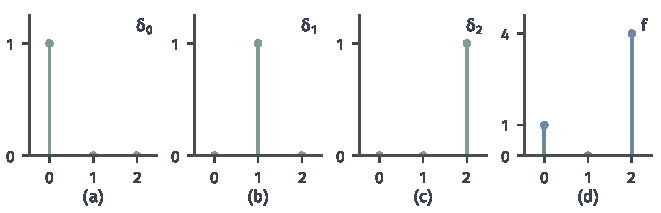
\includegraphics[width=112mm]{figures/04-spaces-measures-and-geometry/03-function-spaces/matplotlib/fvec-indicator-basis/figure.pdf}
  \caption{$X=\{0,1,2\}$上的指示函数基。(a)至(c)是三个基函数$\delta_0,\delta_1,\delta_2$，每个只在一个输入处取$1$。(d)是$f=\delta_0+4\delta_2$，它的三个取值$(1,0,4)$就是坐标。}
  \label{fig:fvec-indicator-basis}
\end{BookInlineFigure}

\paragraph{多项式基与坐标}
有限维函数空间不一定来自有限的输入集合。在整个实轴上考虑$P_m$，即次数不超过$m$的实多项式全体。每个$p\in P_m$可以写成
\[
 p(x)=a_0+a_1x+\cdots+a_mx^m,
\]
所以$1,x,\ldots,x^m$张成$P_m$。

要说明它们是一组基，还须核对线性无关。设$\sum_{k=0}^mc_kx^k$对每个实数$x$都等于零。左边是一个次数不超过$m$的多项式，若系数不全为零，它至多有$m$个根；而它在无穷多个点处取零，所以每个$c_k=0$。于是
\begin{equation}
 \dim P_m=m+1,
 \label{eq:fvec-polynomial-dimension}
\end{equation}
系数$(a_0,\ldots,a_m)$是$p$相对于这组基的坐标。

这个例子把两种“个数”分开了。$P_m$的定义域$\mathbb R$有不可数个点，空间却只有$m+1$维：一旦知道$m+1$个系数，整条曲线在每一点的值都确定了。可以想象一个不可数长的取值列，它的全部分量由$m+1$个数决定。维数只看张成整个空间需要多少方向，与函数定义在多少个点上无关。

在$P_2$上还可以把取值列与系数列的关系算清楚。上一节的$p(x)=2-x+3x^2$，系数列是$(2,-1,3)$。在三个点$0,1,2$处读取值，得到取值列
\[
 p(0)=2,\qquad p(1)=4,\qquad p(2)=12.
\]
一般地，对$a_0+a_1x+a_2x^2$在这三点取值，就是用一个矩阵乘系数列：
\begin{equation}
 \begin{bmatrix}p(0)\\p(1)\\p(2)\end{bmatrix}
 =\begin{bmatrix}1&0&0\\1&1&1\\1&2&4\end{bmatrix}
 \begin{bmatrix}a_0\\a_1\\a_2\end{bmatrix}.
 \label{eq:fvec-vandermonde}
\end{equation}

这个矩阵的行列式等于$(1-0)(2-0)(2-1)=2\neq0$，所以它可逆。这意味着系数列和取值列互相决定，$(2,-1,3)$与$(2,4,12)$只是同一个元素的两列坐标。图~\ref{fig:fvec-coefficient-point}把这三者放在一起：同一条抛物线，在两个坐标系中各是一个点。

\begin{BookInlineFigure}
  \centering
  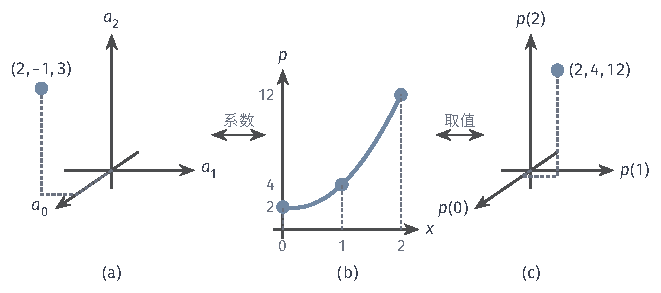
\includegraphics[width=111.919mm]{figures/04-spaces-measures-and-geometry/03-function-spaces/tikz/fvec-coefficient-point/figure.pdf}
  \caption{$P_2$中一个元素的三种面貌。(b)是曲线$p(x)=2-x+3x^2$，蓝点是它在$0,1,2$处的取值。(a)是它的系数列，在以系数为坐标轴的$\mathbb R^3$中是一个点。(c)是它在三点的取值列，在另一个$\mathbb R^3$中也是一个点。两个点由式~\eqref{eq:fvec-vandermonde}的矩阵互相转换。}
  \label{fig:fvec-coefficient-point}
\end{BookInlineFigure}

取值列也可以就是某组基下的坐标，只要选对基。令
\[
 \begin{aligned}
 \ell_0(x)&=\tfrac12(x-1)(x-2),\\
 \ell_1(x)&=-x(x-2),\\
 \ell_2(x)&=\tfrac12x(x-1).
 \end{aligned}
\]
这三个多项式在$0,1,2$上的取值分别是$(1,0,0)$、$(0,1,0)$、$(0,0,1)$，它们在这三点上的行为和指示函数一样。于是
\[
 p=2\ell_0+4\ell_1+12\ell_2.
\]
直接展开右边，得到$(x^2-3x+2)+(-4x^2+8x)+(6x^2-6x)$，合并后正是$2-x+3x^2$。

\subsection{无限维函数空间}
\label{sec:fvec-infinite-dimensional}

有限维向量的长度可以增加：$\mathbb R^1$可以看作$\mathbb R^2$中第二个分量为零的部分，$\mathbb R^2$又可以看作$\mathbb R^3$的一部分，这样一直延续下去。无限维说的是这个过程永远走不到头。若一个线性空间对每个正整数$n$都含有$n$个线性无关的元素，它就不能由任何有限个元素张成，称为\term{无限维}（infinite-dimensional）的。理由是卷二已经证明，由$k$个元素张成的空间中，线性无关的元素至多有$k$个。

\paragraph{全体多项式}
把次数的上限去掉，考虑全体实多项式组成的空间$P=\bigcup_{m\geq0}P_m$。它是线性子空间，因为两个多项式之和仍是多项式。上一小节的论证对每个$m$都成立，$1,x,\ldots,x^m$线性无关，而$m$可以任意大，所以$P$是无限维的。

也可以直接说明任何有限族都张不成$P$。设$q_1,\ldots,q_k$是有限个多项式，其中最高的次数为$d$。它们的任意线性组合次数都不超过$d$，所以$x^{d+1}$不在它们的张成空间中。无论选哪$k$个多项式，总有更高次的多项式落在外面。

\paragraph{全体数列}
数列空间$\mathbb K^{\mathbb N_+}$中，令$e_k$为第$k$项为$1$、其余各项为$0$的数列，称为第$k$个\term{标准单位列}（standard unit sequence），它是$\mathbb K^d$的标准基向量的直接延续。对任意$n$，若$\sum_{k=1}^nc_ke_k$是零数列，读出第$k$项即得$c_k=0$，所以$e_1,\ldots,e_n$线性无关。$n$任意，数列空间是无限维的。

同样的论证说明，只要输入集合$X$有无穷多个点，不同点的指示函数就构成任意多个线性无关的元素，$\mathbb K^X$都是无限维的。这里类比又碰到一个边界：$X$无限时，式~\eqref{eq:fvec-indicator-expansion}不能原样推广。指示函数的有限组合只在有限个点上不为零，所以常数函数$1$不在它们的张成空间中。取值仍然是每个输入上的数，却不再是一组基下的有限坐标。

\paragraph{每个元素有限与整体无限}
无限维并不意味着每个元素都“需要无穷多个方向”。$P$中的每个多项式只用到有限个单项式，它的系数列$[a_0,a_1,\ldots,a_d,0,0,\ldots]$从某一项起全为零；$c_{00}$中的每个数列也只是有限个$e_k$的组合。无限维说的是整个空间：没有一组固定的有限个方向，能同时表示所有元素。

图~\ref{fig:fvec-finite-support-grid}的前三行是三个多项式的系数列，每一行都只占有限个格子，但占到的最靠右的位置没有统一的上限。第四行不同：$e^x$的系数$1/k!$永远不为零。它不是多项式，因为任何多项式求导足够多次后变为零，而$e^x$求导后不变。

\begin{BookInlineFigure}
  \centering
  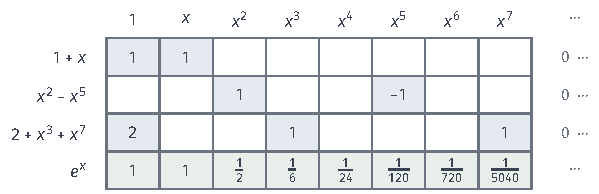
\includegraphics[width=101.469mm]{figures/04-spaces-measures-and-geometry/03-function-spaces/tikz/fvec-finite-support-grid/figure.pdf}
  \caption{系数列的两种形态。每一列对应一个单项式，蓝格是非零系数。前三行是多项式，只占有限个格子，其后全为零，所占范围随元素变化。第四行绿色的$e^x$每一格都不为零，有限个单项式的组合表示不了它。}
  \label{fig:fvec-finite-support-grid}
\end{BookInlineFigure}

数列空间中的常数列$(1,1,\ldots)$与$e^x$处境相同，它不是有限个$e_k$的组合。若想用$e_1,e_2,\ldots$表示这样的元素，就只能借助无穷多项之和，这需要先说明无穷和是什么意思。
